% Pursuing Stacks (cotes 134-2 to 134-8): archive cote 134-2, site page 79 (PDF page 80).
% notes to ch. I. Draft compared: ps1.tex:735-748 ; ps1.tex:958-994 ; ps1.tex:1100-1113.
% AI-transcribed by Claude Opus 5.5 (claude-opus-5-5, adaptive thinking, effort high), Message Batches API, batch ps1 (msgbatch_01Rv5hCaNTtUt4JHx1yqoHPL), 2026-11-12; not yet checked by eye.
\scanpage{134-2/79}
\mspage{53}

(${}^{12}$!)   This is nonsense, as one sees already in the following picture
where  f\hand{$\wedge$}f"= S$_{o}$ :  \hand{\diagram{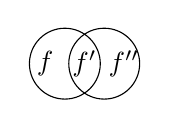
\begin{tikzpicture}\draw (0,0) circle (0.45); \draw (0.5,0) circle (0.45); \node at (-0.25,0) {$f$}; \node at (0.25,0) {$f'$}; \node at (0.75,0) {$f''$};\end{tikzpicture}}}

(${}^{13}$!)   This is nonsense again for n $\geqslant$1,  see PS at the end of section 13.
\margin{Even this PS is still unaccurate, compare comments section 18.}

(${}^{14}$!)   Same mistake as \xout{in} the one noticed in the previous note.  The
fibered products exist in $\underline{C}$\hand{$_{\bullet}$} only,  and \uline{these} should be preserved by the
functors under consideration. Thus the "universal problem" \deleted{\xout{has}} has to be
rephrased somewhat ...

(${}^{15}$)   I guess they are not equivalent,  even when restricting to objects
which are groupoids (i.e. so-called Gr-categories).

(${}^{16}$)  An object of M is called fibrant (resp. trivial) it the map from it
to the final object is fibrant (resp. a weak equivalence).

(${}^{17}$)   This seems doubtful,  unless all objects of M are fibrant (which is
true for the most familiar cases I was having in mind).  But even assuming
this,  we still need a unicity statement (in a suitable sense) for the
functors  $\underline{B}_{o}$\hand{$\to$} M  thus obtained,  in order to be sure that the correspon-%
ding functors  M\hand{$\to$}(Ho) are all canonically isomorphic.  These kind of
questions may be viewed as closely related to the question of existence
(and unicity) of ``test functors'' for a given test category A (here,  the
category of ``standard hemispheres'' \hand{\unsure{$\bigcirc$}}) into a given asphericity or con-%
tractibility structure,  as discussed in section 90 (without yet getting
there \xout{\unsure{the}}\inserted[typed]{any} clear-cut handy existence and unicity theorems \deleted{which are}\inserted{as are} to
be \xout{hoped} hoped for). \inserted{In my notes,} \over{T}{t}he set-up of asphericity and contractibility struc-%
tures,  which has been worked out in the months following,  has been gra-%
dually replacing Quillen's approach to homotopy models.  (I'll have to co-%
me back in due course to the\hand{/}question of the relationship between the two
approaches,  which deserves to be understood.)

(${}^{18}$)  The word ``gerb'' here stands \xout{for} as a ``translation'' of the French
word ``gerbe'',  as used in Giraud's book on non commutative cohomological
algebra.  With the terminology of next section,  we would call it rather
a ``stack of groupoids'' or  ``Gr-stack'' (with a specification by n or $\infty$ if
needed !).

(${}^{19}$!)  This is false,  as seen below.

(${}^{20}$\xout{\unsure{1}}!)  This description is dubious,  as it may give categories $\underline{C}_{n}$ which
are larger than the ones we want.

(${}^{21}$!)  It seems dubious however that the mere category structure of $\underline{C}$ will
allow us to recover the \xout{\unsure{the}} ``primitive'' subcategory $\underline{C}_{o}$ ,  and it looks sa-%
fer to add the latter as an extra structure to $\underline{C}$ .

\mspage{79}
